
\documentclass[article]{memoir}

% ----- Packages -----
\usepackage{amsmath}
\usepackage{amsfonts}
\usepackage{amssymb}
% Must come after amsmath.
%\usepackage{amsthm}

\usepackage{mathtools}
\usepackage{subdepth}
\usepackage{dsfont}
\usepackage{flafter}
\usepackage{graphicx}
\usepackage{listings}

% ----- Page -----
\setlrmarginsandblock{1in}{1in}{*}
\setulmarginsandblock{1in}{1in}{*}
\checkandfixthelayout

\makepagestyle{name}
    \makeevenhead{name}{\textsl\thetitle}{}
    {\textsl{\thepage\ of \thelastpage\ --- Nick Ulle}}
    \makeoddhead{name}{\textsl\thetitle}{}
    {\textsl{\thepage\ of \thelastpage\ --- Nick Ulle}}
\makepagestyle{no-name}
    \makeevenhead{no-name}{\textsl\thetitle}{}
    {\textsl{\thepage\ of \thelastpage}}
    \makeoddhead{no-name}{\textsl\thetitle}{}
    {\textsl{\thepage\ of \thelastpage}}

% ----- Floats -----
\changecaptionwidth
\captionwidth{0.6\textwidth}
\setfloatadjustment{table}{\centering}
\setfloatadjustment{figure}{\centering}

\newsubfloat{table}
\newsubfloat{figure}

%\setFloatBlockFor{chapter}

% ----- Listings -----
\lstset{basicstyle = \ttfamily, numberstyle = \tiny, stepnumber = 2}

% ----- Commands -----
% Unbind some things that are never useful.
    % Built-in probability operator:
\let\Pr\relax%
    % Slashed O:
\let\O\relax%

% Set up sentence-ending ellipses.
\def\ldotsplus{\mathinner{\ldotp\ldotp\ldotp\ldotp}}
\def\fourdots{\relax\ifmmode\ldotsplus\else$\m@th \ldotsplus\,$\fi}

% Use the nice phi.
\let\temp\phi
\let\phi\varphi
\let\varphi\temp


\DeclareMathOperator{\Pr}{\mathds{P}}
\DeclareMathOperator{\E}{\mathds{E}}
\DeclareMathOperator{\Var}{Var}
\DeclareMathOperator{\Cov}{Cov}
\DeclareMathOperator{\Cor}{Cor}
\DeclareMathOperator{\eul}{e}
\DeclareMathOperator{\1}{\mathbf{1}}
\DeclareMathOperator{\sign}{sign}
\DeclareMathOperator{\diag}{diag}
\DeclareMathOperator{\tr}{tr}
\DeclareMathOperator*{\argmin}{argmin}
\DeclareMathOperator*{\argmax}{argmax}
\DeclareMathOperator{\O}{\mathcal{O}}
%\DeclareMathOperator{\N}{N}
%\DeclareMathOperator{\F}{F}
%\DeclareMathOperator{\Wishart}{W}

\newcommand{\abs}[1]{\lvert#1\rvert}
\newcommand{\norm}[1]{\lVert#1\rVert}
\newcommand{\ceil}[1]{\lceil#1\rceil}
\newcommand{\floor}[1]{\lfloor#1\rfloor}
\newcommand{\df}{\,\mathrm{d}}
\newcommand{\pd}[2][]{\frac{\partial#1}{\partial#2}}
\newcommand{\dv}[2][]{\frac{\mathrm{d}#1}{\mathrm{d}#2}}
\newcommand{\inD}{\mathop{\overset{\mathrm{d}}{\longrightarrow}}}
\newcommand{\inP}{\mathop{\overset{\Pr}{\longrightarrow}}}
\newcommand{\qed}{\hfill \ensuremath{\square}}
\newcommand{\T}{^\mathsf{T}}
\newcommand{\C}{^\mathsf{C}}
\newcommand{\io}{\text{ i.o.}}
\newcommand{\ev}{\text{ ev.}}
\newcommand{\dist}[1]{\operatorname{#1}}
\newcommand{\iid}{\overset{\mathrm{iid}}{\sim}}
\newcommand{\on}[1]{\operatorname{\mathds{1}}\!\left\{#1\right\}}
\newcommand{\ind}{\protect\mathpalette{\protect\independenT}{\perp}}

\def\independenT#1#2{\mathrel{\rlap{$#1#2$}\mkern4mu{#1#2}}}


\pagestyle{name}
\title{STA 250: Homework 2}

\begin{document}
\chapter*{Report}
\begin{enumerate}
\item
The bootstrap estimates the standard error of a statistic by resampling from
the empirical distribution.
This is especially useful where deriving an analytic estimator of the standard
error is unwieldy.
When the number of observations, $n$, in the data set is very large, the
bootstrap is no longer computationally feasible.
The bag of little bootstraps works by drawing $s$ subsamples of size $b$ from
the data set, without replacement. 
From each subsample, $r$ bootstrap samples of size $n$ are resampled with
replacement.
This produces $s$ bootstrapped standard errors, which can be averaged to get
an overall estimate.

The key advantage to this approach is that there are at most $b$ unique
observations in each bootstrapped sample.
Provided the statistic of interest can be computed from weighted observations,
this means only $b$ weighted observations need to be used in its computation,
rather than a full $n$ observations.
The result is a considerable savings on computation time.

This assignment used $s = 5$, $r = 50$, and $b = n^{0.7}$.
The algorithm appears to have performed well on the supplied data set.
Based on the index plot (figure~\ref{fig:index}), almost all of the estimated
standard errors fall within $0.01 \pm 0.001$.
Performance of the code was acceptable, with each job running about $8$
minutes at most.

\item
The mapper script, mapper.py, does most of the work in this MapReduce.
It maps each $(x, y)$ pair to a bin of size $0.1 \times 0.1$ by multiplying
both by $10$, taking the floor and ceiling, and then dividing these by $10$.
The floored result gives $(x_{\mathrm{lo}}, y_{\mathrm{lo}})$, 
while the ceilinged result gives $(x_{\mathrm{hi}}, y_{\mathrm{hi}})$.
These are then combined into a key.
The key is output with the value $1$, but this value is not actually
necessary (the reducer script could just assume it is always $1$).

The reducer script, reducer.py, counts the number of times it receives each
key (and does respect the supplied value), outputting the results in
comma-separated format.

After a few false-starts due to a bad choice of hashbang,
the entire map-reduce took about an hour on Amazon, using $1$ ``large'' master
core and $2$ ``large'' compute cores.
This was satisfactory considering the size of the data set and the amount of
time spent waiting for enough capacity on the class account to create the 
cluster.
The resulting two-dimensional histogram (figure~\ref{fig:hist}) was a good
reward.

It was surprising to me that NumPy had no built-in function to floor or ceiling
a number to arbitrary precision.
It was also very nice how painless it was to get everything to work.
That said, the error feedback from Hadoop was not very illuminating with
regards to my hashbang problem. 
Presumably Hadoop keeps logs of the actual errors the map-reduce produces?
These would be tremendously useful in diagnosing a failed map-reduce.

\item
Using Hive was slightly more tricky than the other parts of the assignment,
because few instructions were provided (not even the layout of the data).
It took about an hour of experimenting with Hive and the mini data set on the
Amazon cluster to figure out what to do.
The difficulty was not in writing the SQL to create the table, but in
determining whether the data had to be copied into Hadoop, or could be used
directly from the S3 bucket.
The former proved more fruitful.
Once that was sorted, running the actual job on a fresh cluster took
approximately 10 minutes (see figure~\ref{fig:mean-var} for the resulting plot).

\end{enumerate}
    \begin{figure}[p]
    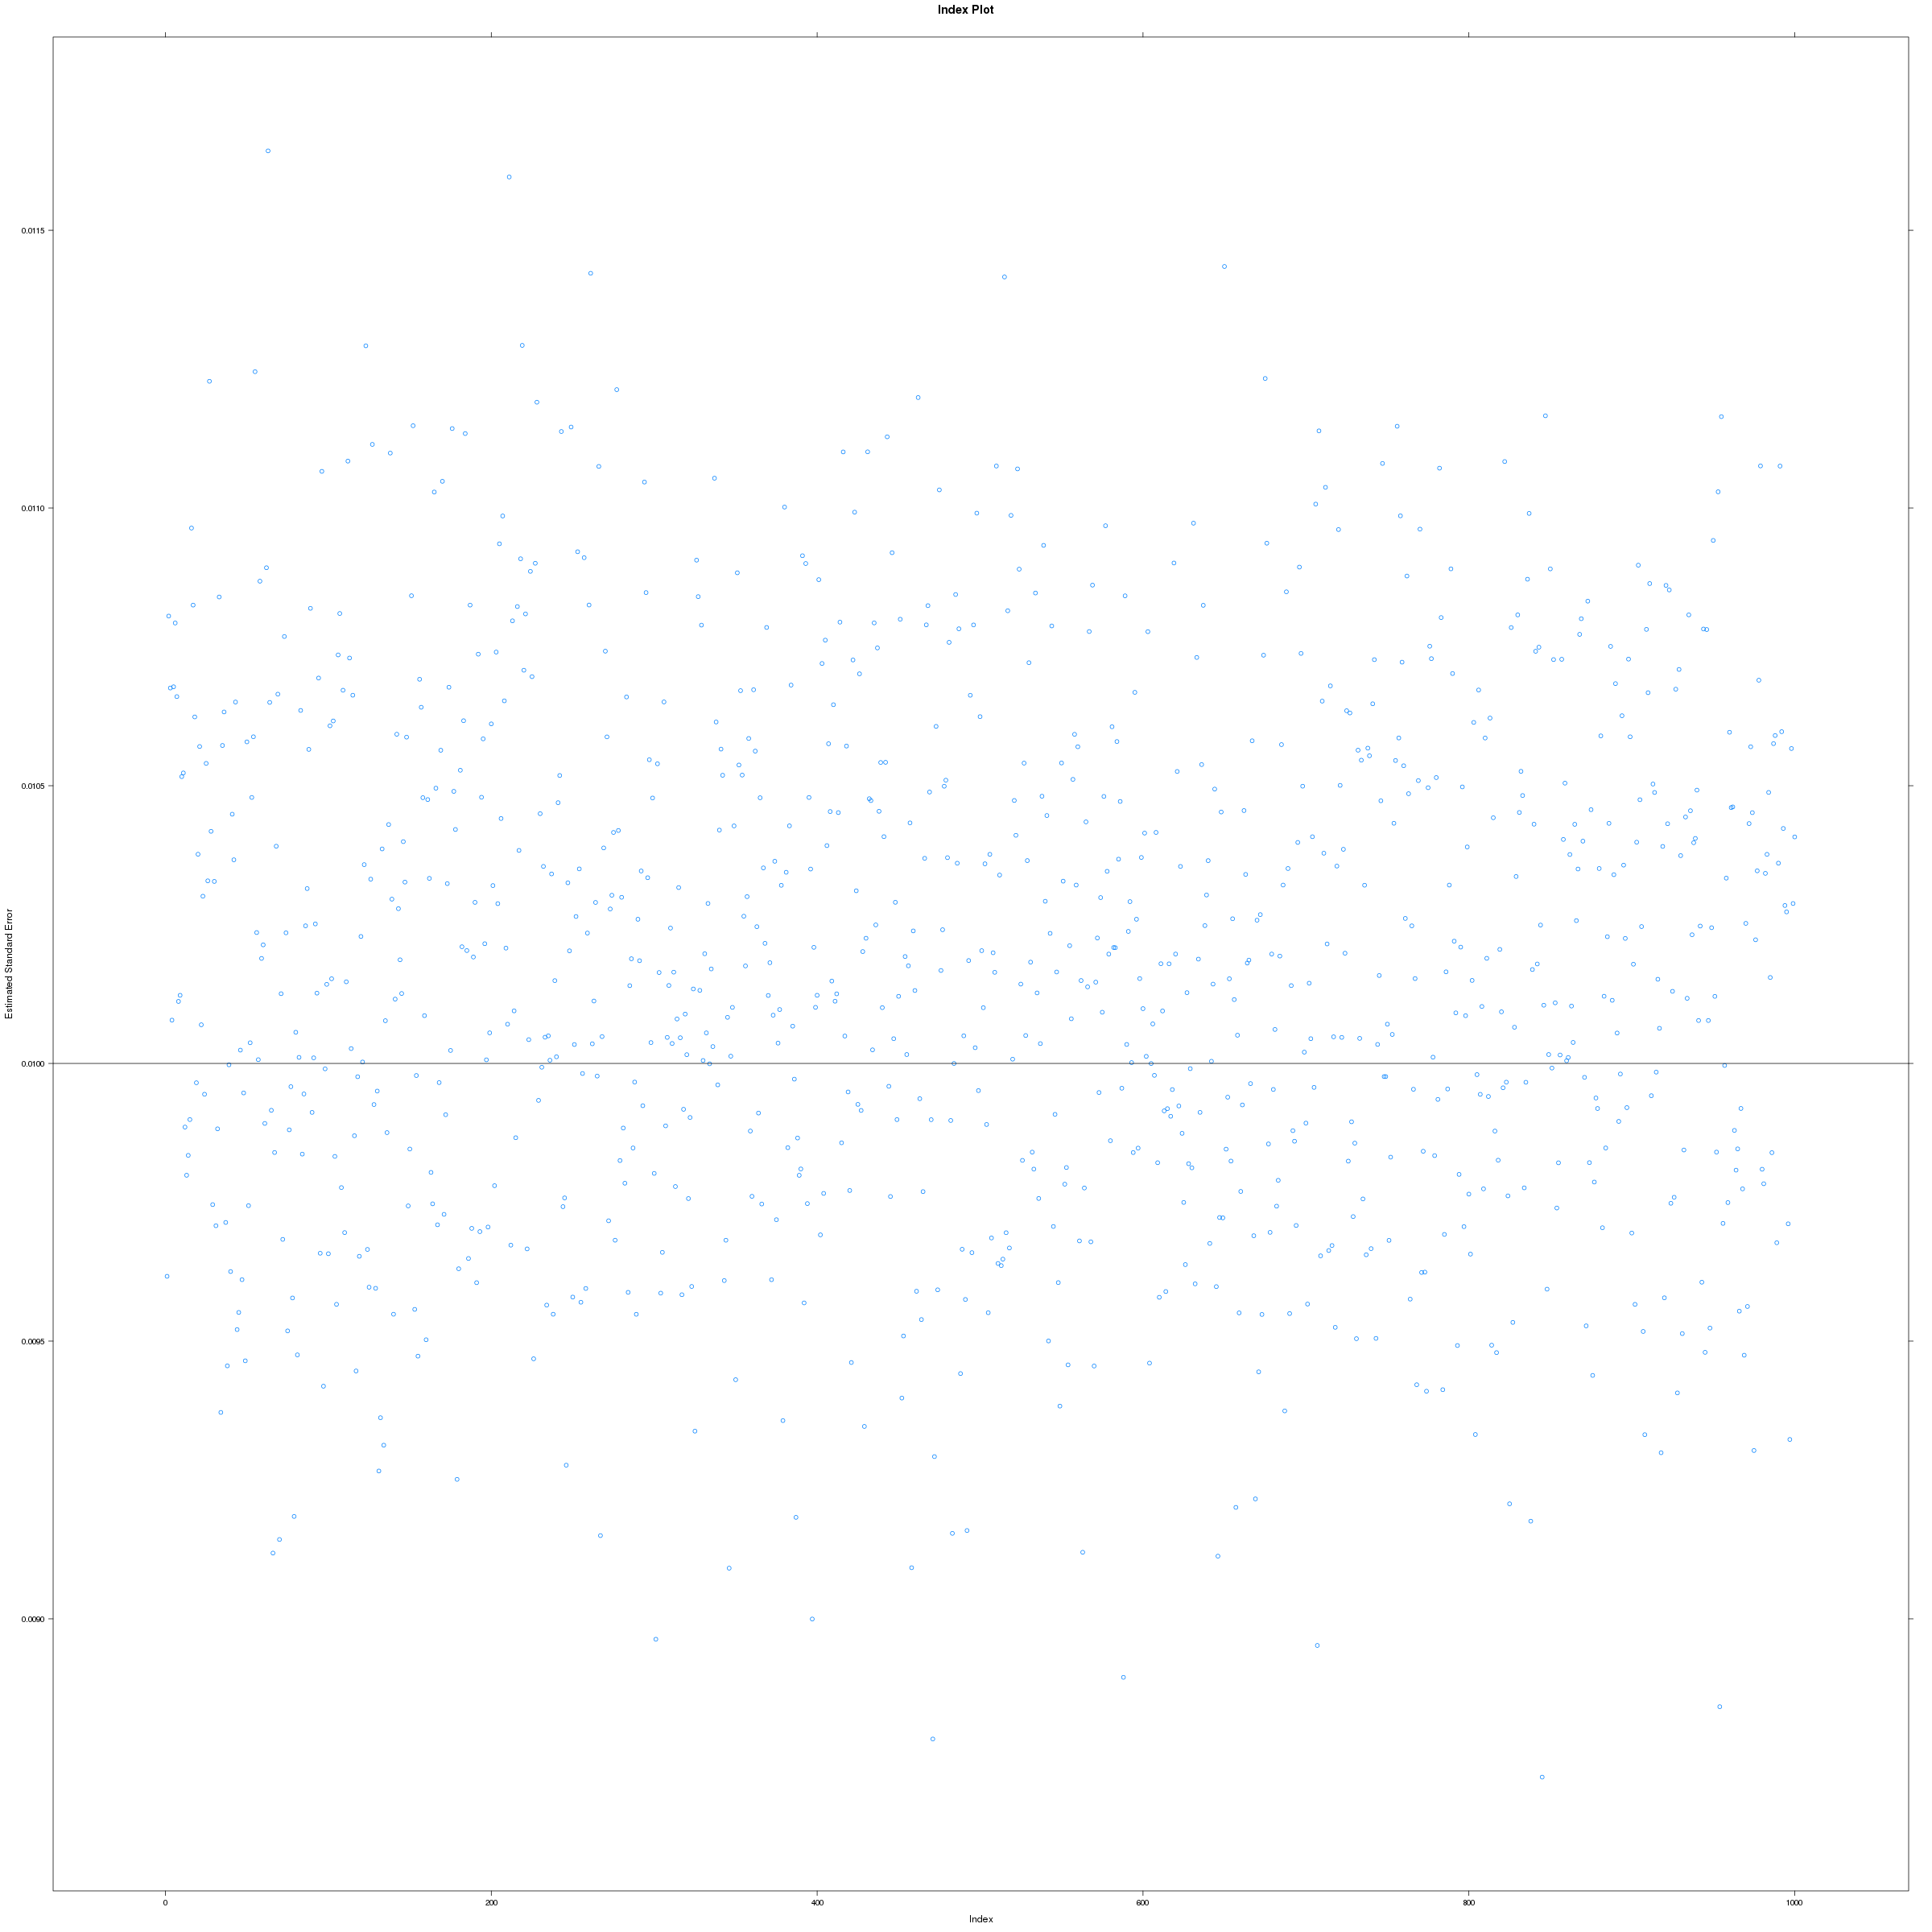
\includegraphics[width = 0.9\textwidth]{res/01_index_plot.png}
    \caption{Plot of estimated standard error against parameter index.}
    \label{fig:index}
    \end{figure}

    \begin{figure}[p]
    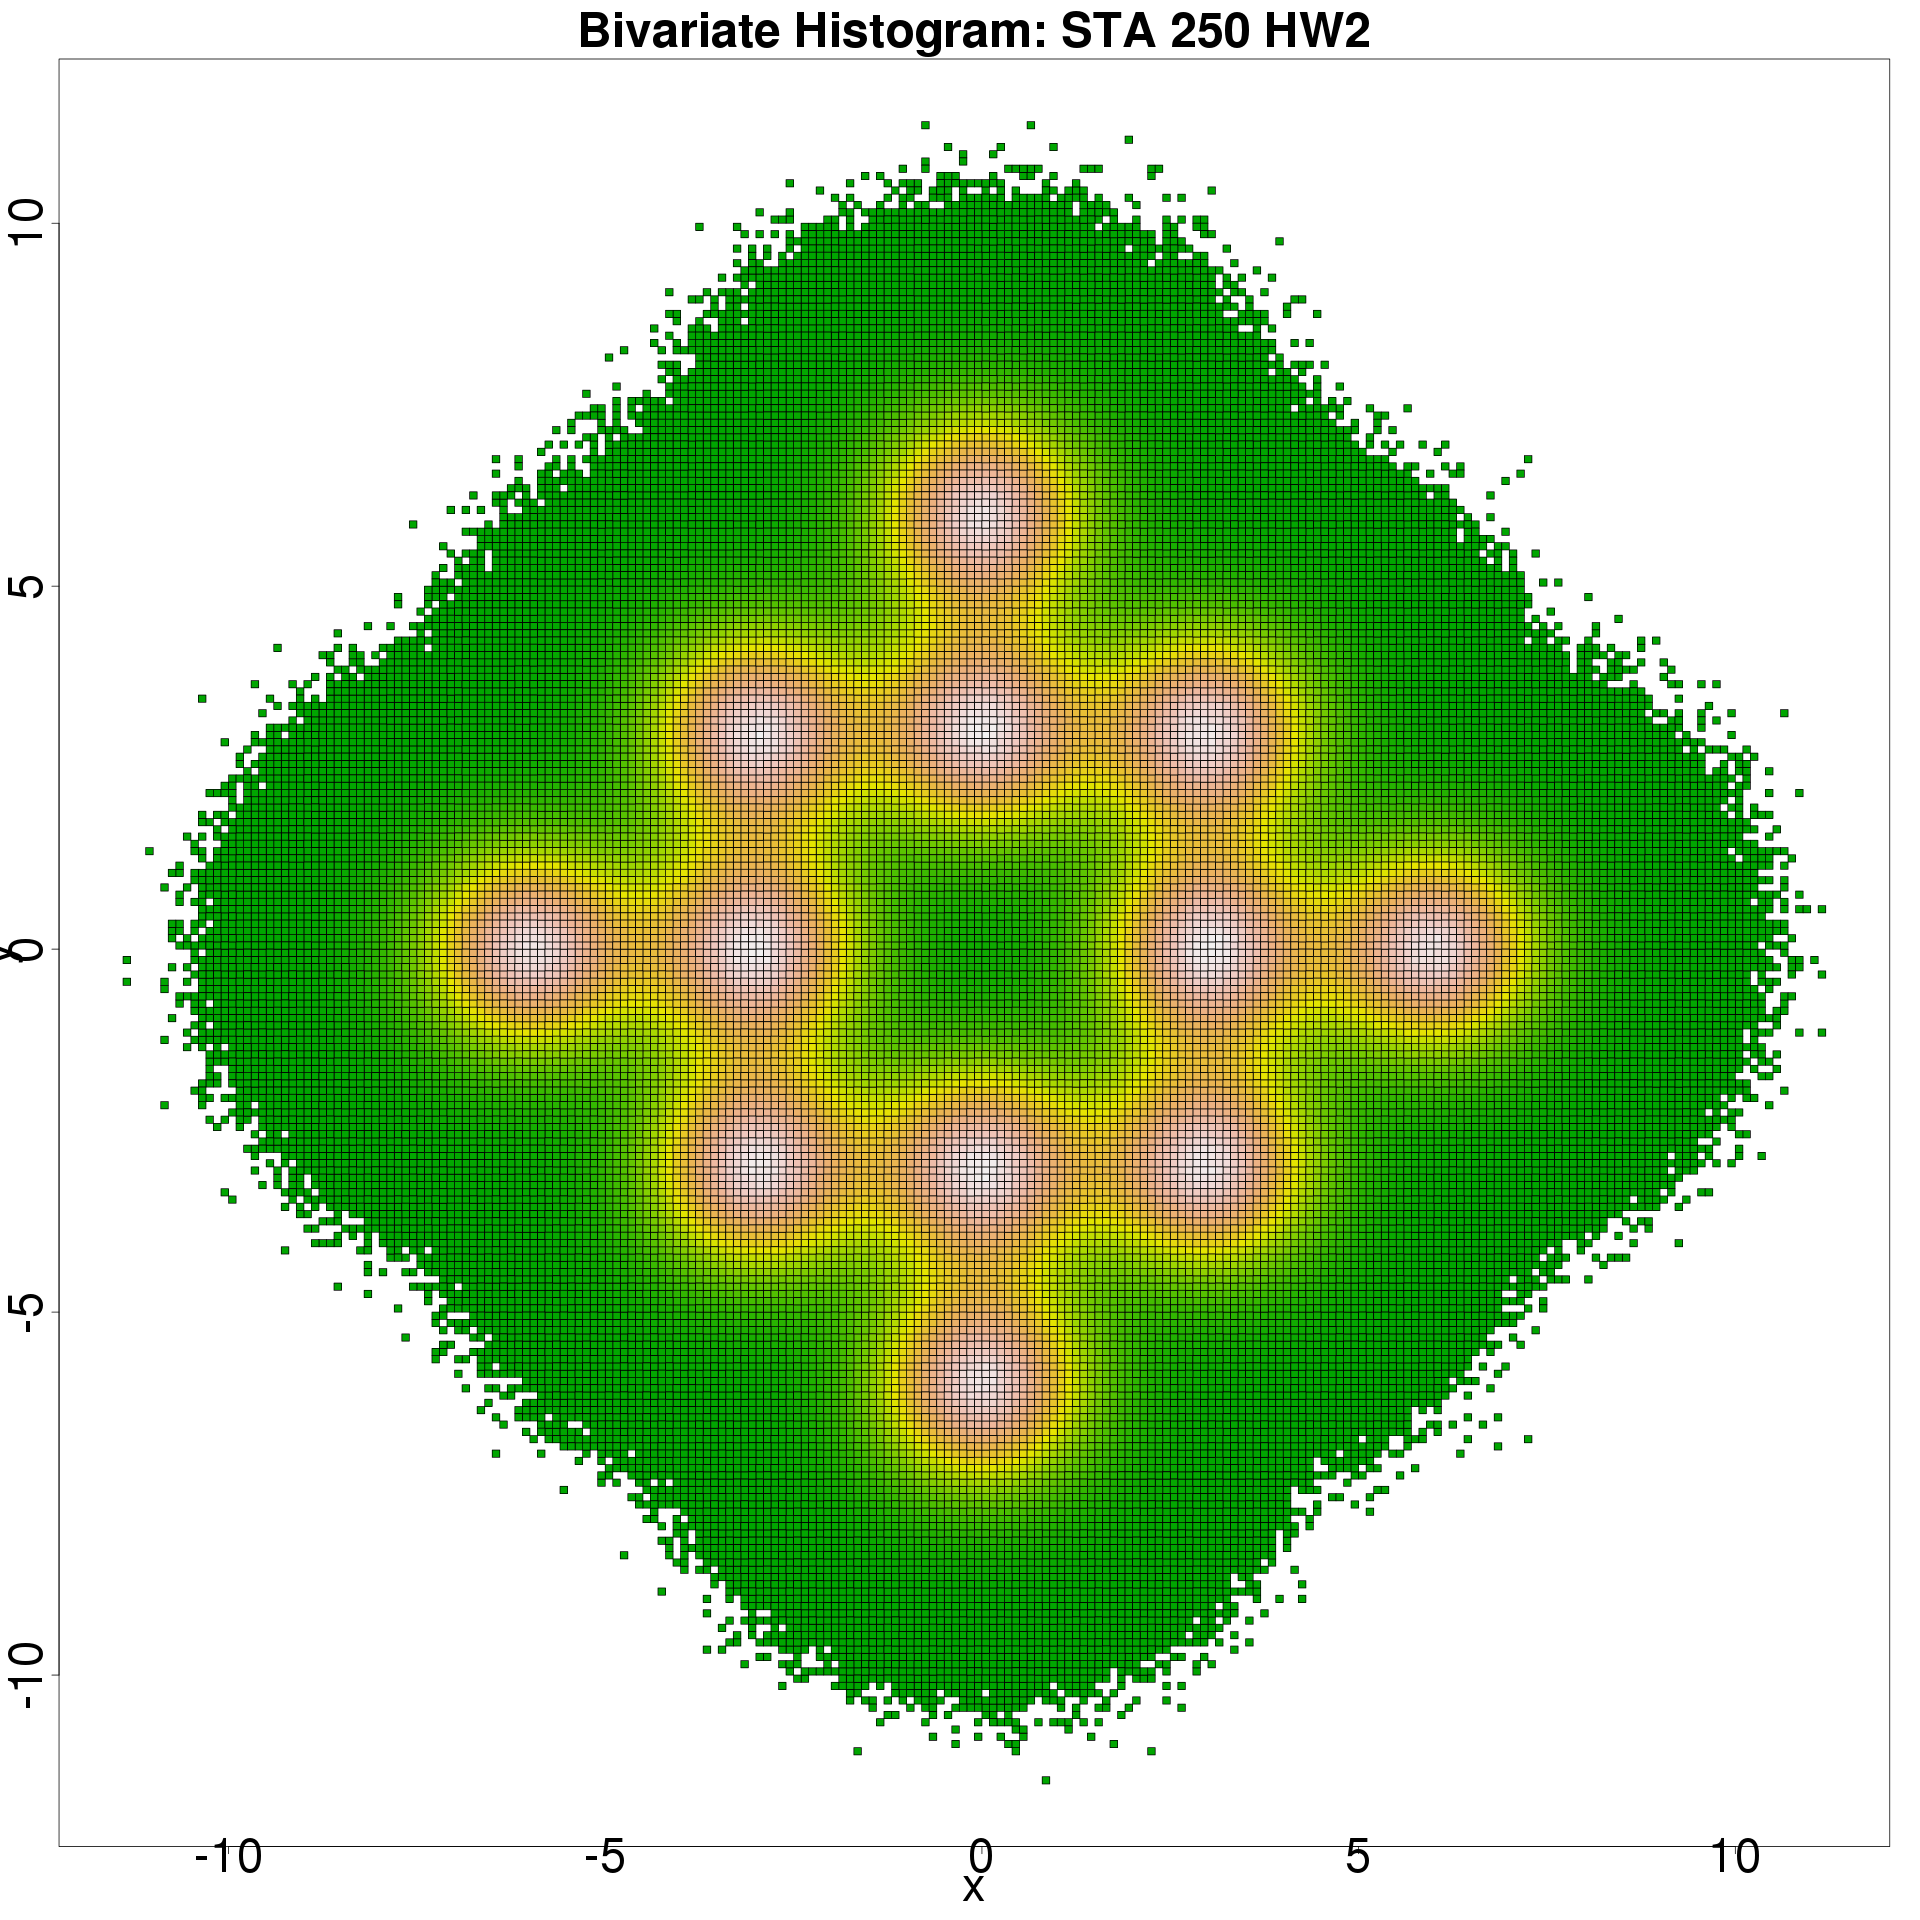
\includegraphics[width = 0.9\textwidth]{res/hist2d.png}
    \caption{
    Two-dimensional histogram resulting from binning the supplied data.
    }
    \label{fig:hist}
    \end{figure}

    \begin{figure}[p]
    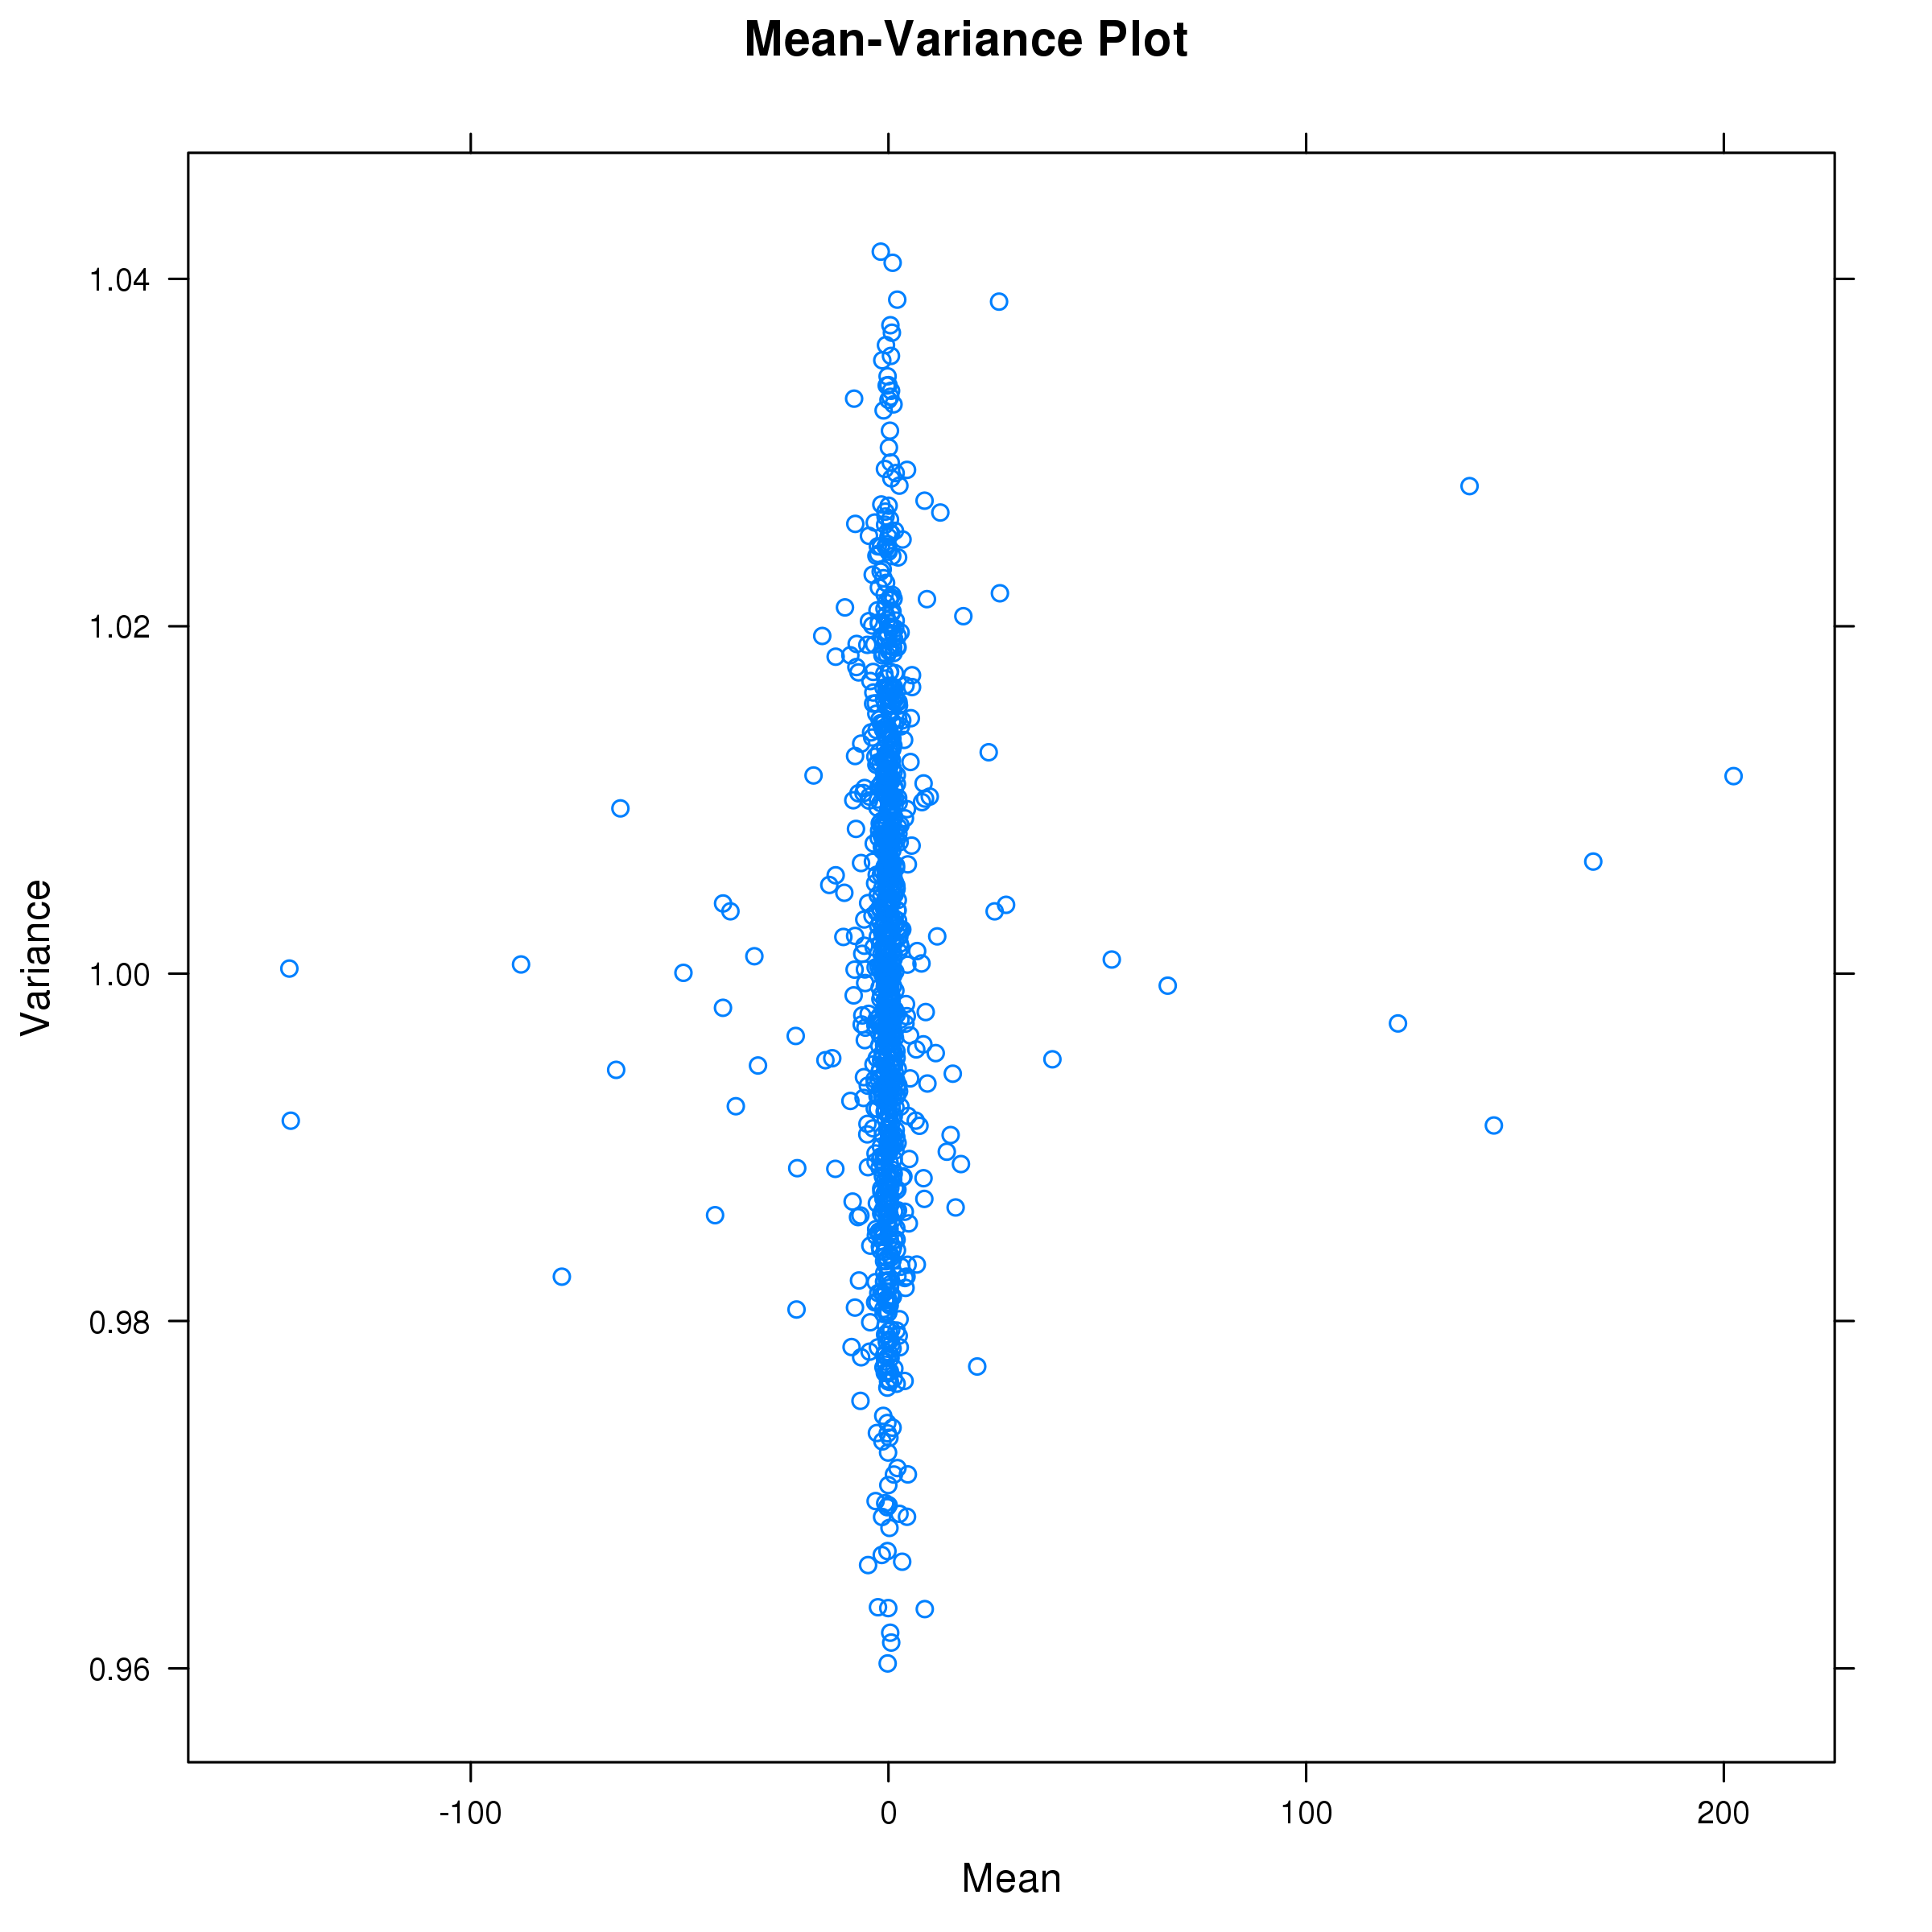
\includegraphics[width = 0.9\textwidth]{res/03_mean_var_plot.png}
    \caption{
    Plot of within-group means against within-group variances for the 
    supplied data.
    }
    \label{fig:mean-var}
    \end{figure}

\clearpage
\chapter*{Source Code}
\hrule
\lstinputlisting{../BLB/BLB_lin_reg_job.py}
\hrule
\lstinputlisting{../BLB/BLB_index_plot.R}
\hrule
\lstinputlisting{../Streaming/mapper.py}
\hrule
\lstinputlisting{../Streaming/reducer.py}
\hrule
\lstinputlisting{../Hive/mean_var.sh}
\hrule
\lstinputlisting{../Hive/mean_var.sql}
\hrule
\lstinputlisting{../Hive/plot_mean_var.R}
\end{document}

